\documentclass[journal]{IEEEtran} % use the `journal` option for ITherm conference style
\IEEEoverridecommandlockouts
% The preceding line is only needed to identify funding in the first footnote. If that is unneeded, please comment it out.
\usepackage{cite}
\usepackage{amsmath,amssymb,amsfonts}
\usepackage{algorithmic}
\usepackage{graphicx}
\usepackage{textcomp}
\usepackage{xcolor}
\def\BibTeX{{\rm B\kern-.05em{\sc i\kern-.025em b}\kern-.08em
    T\kern-.1667em\lower.7ex\hbox{E}\kern-.125emX}}

\usepackage{tikz}
\usetikzlibrary{shapes.geometric, arrows.meta, positioning, shadows.blur}

\tikzstyle{process} = [
    ellipse,
    minimum width=5.3cm,
    minimum height=0.9cm,
    text centered,
    draw=blue!60,
    fill=blue!12,
    font=\small,
    blur shadow={shadow blur steps=5}
]

\tikzstyle{arrow} = [
    thick,
    ->,
    >=Stealth,
    draw=blue!70
]

\usepackage{booktabs}
\usepackage{array}
\usepackage{xcolor}

% MUST be last
\usepackage[
    pdfborder={0 0 0},
    colorlinks=false,
    breaklinks=true
]{hyperref}

\setlength{\tabcolsep}{18pt}      % horizontal padding


\begin{document}


\title{\Huge IoT Drift: Catch Me If You Can}

\author{
\begin{tabular}{c c}
\large Marina Melkonyan & \large Gurgen Hovakimyan \\[0.3cm]

\normalsize BS in Data Science &
\normalsize Adjunct Lecturer \\

\normalsize American University of Armenia &
\normalsize American University of Armenia \\

\normalsize \texttt{marina.melkonyan@edu.aua.am} &
\normalsize \texttt{ghovakimyan@aua.am}
\end{tabular}
}

\date{}

\maketitle


\begin{abstract}

\textbf{Long term IoT sensor networks continuously collect data that powers modern intelligent systems. However, as time passes, environmental changes, hardware aging, lighting conditions, weather patterns, and other real world factors can gradually alter the data being produced. These hidden shifts in feature distributions, known as feature drift, often remain unnoticed while silently reducing the reliability of machine learning models. This capstone investigates hidden feature drift in continuous IoT imagery streams using three real world long term datasets: urban streetlight camera imagery, agricultural orchard monitoring from Raspberry Pi sensors, and pest monitoring sticky trap cameras. Together, these datasets span multiple years, diverse environments, and different sensor types, enabling robust cross domain evaluation. Unsupervised deep learning methods, including variational and convolutional autoencoders, were trained on stable baseline periods and evaluated on later target periods to identify drift through reconstruction loss and latent distribution changes without requiring labeled data. To improve trustworthiness, the project combines multiple model architectures, custom drift metrics, statistical testing, and metadata based validation to distinguish genuine environmental drift from temporary anomalies or sensor artifacts. Results show that hidden drift can be detected accurately and often rapidly, while detection performance depends on both domain differences and environmental variability. Overall, this research contributes an end-to-end, practical drift monitoring pipeline that is interpretable, transferable across domains, and suitable for long-running real-world IoT deployments.}


\end{abstract}

\begin{IEEEkeywords}
Internet of Things, Feature Drift Detection, Autoencoder, Reconstruction Loss, Latent Space, Image Streams, Seasonal Drift}
\end{IEEEkeywords}

\section{INTRODUCTION}

Internet-of-Things (IoT) systems operate by continuously collecting data from distributed sensors deployed in dynamic real-world environments. As these environments evolve, the characteristics of the generated data streams also change over time due to factors such as weather conditions, sensor aging, hardware recalibration, and shifts in usage patterns. As a result, IoT data streams rarely remain statistically stable. This evolving nature of the data leads to feature drift, a subtype of concept drift where patterns learned from historical data no longer accurately represent current observations. In such settings, machine learning models that assume fixed data distributions tend to lose predictive accuracy over time, which directly affects the reliability and trustworthiness of long-term IoT analytics. Consequently, identifying and managing concept drift has become a central challenge in deploying robust learning systems for continuous IoT data streams\cite{one}.

Previous research has extensively studied concept and feature drift detection in streaming data, proposing statistical, window-based, and weighting-based approaches to identify distributional changes in sensor measurements and derived features\cite{two,three}. Recent studies in IoT contexts demonstrate the effectiveness of unsupervised drift detection methods to identify drift in sensor signals and image-based streams, but evaluations are often limited to detection performance on generic benchmarks or isolated sensor modalities\cite{four,five, six, ten}.

Despite substantial progress, there remains a gap in integrated approaches that monitor feature drift in high-dimensional IoT data streams using unsupervised methods\cite{three, four, ten}, and validating the underlying causes of detected drift. Most existing studies focus on detection accuracy, while limited attention is given to understanding how drift can be minimized based on different environments and how detected drift events can be validated against physical or environmental changes. This project aims to address this gap by applying unsupervised drift detection techniques to different real-world IoT imagery datasets, to find suitable metrics for systematically analyzing feature drift behavior, and introducing a validator mechanism to improve the reliability and interpretability of continuous IoT data stream analytics.

\subsection*{Research Questions}
\begin{enumerate}
    \item How does the mean time to detection (MTTD) of the validator change when applied to cross-domain data streams compared to its baseline performance in the source domain?
    \item What is the sensitivity of unsupervised reconstruction loss as a trigger for drift adaptation in IoT imagery, and how does this sensitivity correlate with the degree of environmental variance across long-term data streams?
\end{enumerate}
\end{subsection*}

\section{Literature Review}

A 2024 systematic review covering more than 200 studies on online learning in evolving data streams \cite{one} revealed an important gap between research advances and real-world deployment. While many drift detection methods perform well in controlled academic settings, they are often evaluated on balanced, low-dimensional, and labeled datasets. In contrast, real IoT systems produce continuous streams of high-dimensional sensor data that are typically unlabeled and frequently imbalanced, making drift detection far more challenging in practice \cite{one,two}. The review specifically points to the need for \textbf{unsupervised} multivariate approaches that can handle complex sensor data such as imagery, which closely matches the focus of this research. Further research exploring how different weighting strategies influence detector sensitivity and response time shows that methods based on fixed windows often struggle when the strength of drift changes over time. Despite this fact, adaptive approaches remain more stable and responsive. These findings reinforce the design choices made in this study and highlight the need for more flexible drift detection methods. In response, this research uses adaptive kernel bandwidth selection through the median heuristic in the \textbf{STKA} metric, together with bootstrap-based confidence intervals, allowing drift to be assessed more reliably than with fixed thresholds alone.

Recent research shows that \textbf{VAE} brings a structural advantage for IoT drift detection beyond mere dimensionality reduction\cite{six}: because the encoder is trained to map inputs onto a regularized Gaussian prior, samples from a shifted distribution produce latent codes that deviate measurably from that prior, generating elevated reconstruction error and measurable distribution changes simultaneously. Research on IoT sensor calibration demonstrated that a VAE trained on clean sensor readings can detect and quantify drift caused by hardware aging through the reconstruction loss even without any labeled degradation examples\cite{six}. The core mechanism is motivated from what is used here, however, the approach is changed. The \textbf{novel} solution suggested in this research is based on a simple but yet powerful idea: train different \textbf{autoencoder architectures} on a reference periods, then watch how hard they struggles to reconstruct images from a later period. If reconstruction gets difficult, we deal with \textbf{drift}.

Additionally, drift in IoT sensor networks presents challenges that extend beyond what generic streaming benchmarks capture. One of the most practically focused studies in this space demonstrated analytics tailored to heterogeneous IoT sensor networks, combining statistical window tests with sensor-level metadata validation to distinguish environmental drift from sensor faults \cite{five}. The key finding was that drift detected purely from data streams is frequently confounded by transient sensor anomalies like power fluctuations, calibration resets, and that correlating detected events with maintenance logs and environmental metadata dramatically reduces the false positive rate. The \textbf{validater module} in this capstone operationalizes this principle by cross-referencing detected latent drift with brightness changes, GPS consistency, fault detection rates, and confidence score shifts.

Moreover, research on concept drift localization in IoT intrusion detection streams \cite{seven} introduced the idea of decomposing a detected drift event into contributions from individual feature subsets rather than producing a single global alarm. This enables targeted remediation by identifying where in a feature space drift is concentrated. It is also worth noting that similarity metrics across neural network representations \cite{thirteen} provide a useful theoretical grounding for why latent-space comparisons are meaningful: when two distributions of latent codes diverge, they are likely encoding genuinely different visual content rather than superficially different pixels. Finally, the streetlight dataset \cite{eleven}, the pomegranate orchard time series \cite{fourteen}, and the stink bug trap imagery\cite{fifteen} are each assembled for real-world monitoring contexts, providing the kind of messy, domain-specific conditions, which is exactly what makes them useful here. Real sensors break, lighting changes, traps get replaced, and trees grow; a drift detection pipeline that cannot cope with that kind of noise is not much use in practice\cite{one, two}.

Taken together, \textbf{three gaps} emerge from the literature that this work directly targets. Existing drift detectors are rarely tested across genuinely heterogeneous IoT deployments, leaving their cross-domain generalisability largely unknown\cite{three,four,ten}. Studies also rarely measure how quickly drift is caught or how \textbf{detection sensitivity shifts} with environmental variability, giving practitioners no principled basis for tuning thresholds in new settings\cite{one,two}. Finally, detected drift signals almost never get cross-checked against physical context, making it hard to tell real distributional change apart from transient noise like lighting fluctuations or hardware faults\cite{five,seven}. This research closes all three gaps: multiple autoencoder architectures are trained on three real-world datasets with detection speed quantified via MTTD; a systematic sensitivity analysis links reconstruction error to environmental variance metrics; and a validator module cross-references latent drift with sensor metadata to produce trustworthy, interpretable alerts---bridging the divide between controlled benchmarks and the messy reality of long-running IoT deployments.

\section{Methodology}

In this section, we walk through how the problem of detecting and quantifying feature drift in IoT sensor imagery is approached without ever needing a single labeled example of what drift actually looks like. The pipeline is designed to be end-to-end: starting from raw images and metadata, moving through feature extraction and model training, and ending with a validated drift score that operators can act on.

\begin{figure}[htbp]
\centering
  \includegraphics[width=0.58\textwidth]{Figuras/pipe.jpg} 
  \caption{End-to-end feature drift monitoring pipeline}
\end{figure}

\subsection{Datasets and Study Design}

Three real-world IoT camera datasets are used, each posing a different kind of challenge for drift detection.

The first and primary dataset comes from a network of fixed urban streetlight cameras that have been operating continuously for four years\cite{eleven}. Each image arrives with rich metadata:the captured timestamp, GPS coordinates, hardware fault flags, a model confidence score, and a daytime/nighttime label. To study seasonal drift, winter images (January–March, Q1) are treated as the reference period and summer images (July–September, Q3) as the target. This pairing maximizes environmental contrast in lighting conditions, color temperature, and vegetation are dramatically different across these windows, while the cameras themselves remain physically unchanged, making it an ideal tested. A \textbf{daytime/nighttime split} is applied as a secondary robustness check to confirm that any detected drift is not merely an artefact of changing daylight hours.

The second dataset comes from cameras monitoring individual pomegranate trees across two growing seasons\cite{fourteen}. Unlike the streetlight case, each camera watches a different physical tree, so drift must be evaluated per sensor rather than globally: pooling all cameras together would mix genuinely drifting sensors with stable ones and obscure the picture.

Finally, the third dataset is a single camera monitoring an insect sticky trap over one complete field season\cite{fifteen}. Here, the summer period (Q3) acts as the reference and autumn (Q4) as the target. This dataset presents a unique complication: the physical trap is replaced multiple times during the season, each replacement resetting the visual appearance of the monitored surface. A core methodological challenge is therefore to distinguish genuine \textbf{seasonal drift} from these sudden trap-change artefacts.

\subsection{Feature Extraction: Two Approaches and Why They Differ}

For all three datasets the first step is constructing a structured catalogue that associates every image with its capture timestamp, sensor identity, and any available metadata. The catalogue is the single source of truth for all downstream indexing: when images are loaded for feature extraction, for training, or for inference, they are always accessed through the catalogue rather than through raw directory scans, which ensures that features and metadata rows remain aligned throughout the pipeline.

Images are split by temporal period to use one period for training and the other for target drift identification. For Dataset 1 the split criterion is calendar quarter (Q1 = January–March, Q3 = July–September). For Dataset 2 it is year (2021 reference, 2022 target) and for Dataset 3 it is again calendar quarter (Q3 reference, Q4 target). Temporal metadata is enriched after loading by computing derived fields day of year, month, day of week which are used in validation and decomposition later.

Before any model can learn what "normal" looks like, it needs a compact numerical description of each image. Two different approaches are used across the datasets, reflecting a natural evolution in the pipeline as the problem grew more demanding.

In Dataset~1's early iterations we use \textbf{RGB Histogram Feature extraction} method, during which for each color channel a 256-bin histogram is computed over the normalized $[0,1]$ pixel range and then normalized to sum to~1. The three channel histograms are concatenated into a single 768-dimensional vector. This representation captures the overall color distribution of an image cheaply, without any GPU requirement, and is invariant to spatial layout. However, its weakness is that it knows nothing about objects or structure: two images with the same color palette but completely different content would look identical to the histogram.

\begin{figure}[htbp]
  \centering
  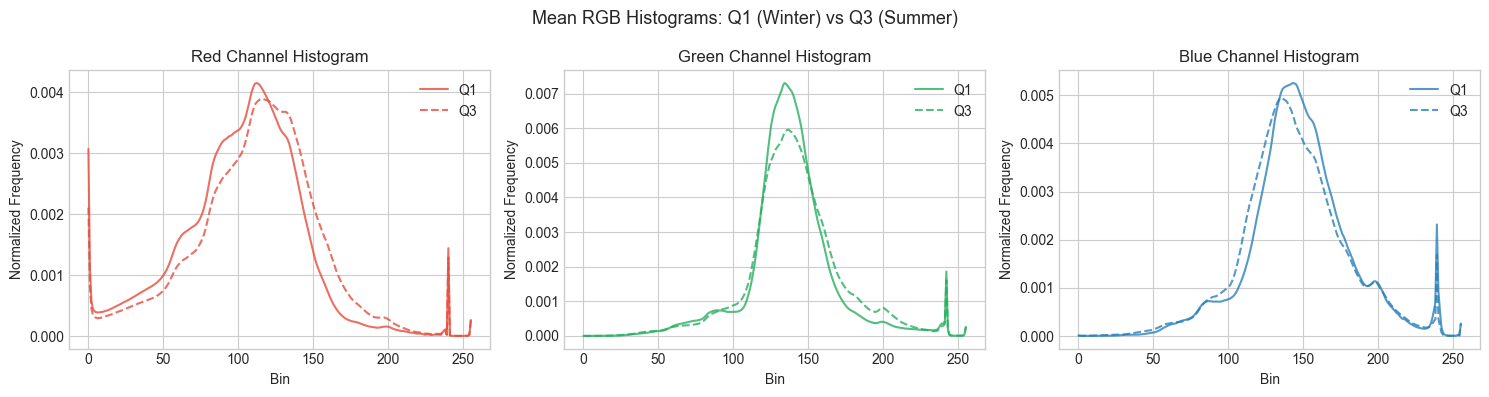
\includegraphics[width=0.5\textwidth]{Figuras/rgb.png} 
  \caption{Mean RGB Histograms:Q1(Winter) vs Q3(Summer)}
\end{figure}


To overcome this limitation, later pipeline versions replace histograms with features extracted from a \textbf{ResNet18} network pretrained on \textbf{ImageNet}\cite{thirteen}. The 512-dimensional activation vector from the penultimate layer encodes mid-level semantic content like textures, shapes, object parts that a histogram cannot capture. For Datasets 2 and 3, where the subject matter (individual trees, sticky traps) demands spatial awareness, a convolutional autoencoder architecture processes the raw image pixels directly through successive convolutional blocks with batch normalisation, ReLU activations, and max pooling, producing a 128-dimensional latent vector.

The key insight in this choice is that richer features come at a cost: CNN features are higher-dimensional and require more data and compute to model reliably. For the large streetlight dataset this trade-off is clearly worthwhile; for the smaller per-tree and sticky-trap datasets it is managed by keeping the architecture convolutional end-to-end so that spatial patterns are preserved.

\subsection{Autoencoder Training and Drift Quantification}
With features in hand, the next question is: how do we actually measure drift? The answer, consistent across all three datasets, is an autoencoder trained solely on reference-period images. The intuition is simple: once the model has learned what ``normal'' looks like, passing target-period images through it will produce higher reconstruction error wherever those images deviate from the reference distribution. That reconstruction error is our operational definition of drift \cite{nine}.

The first model explored and chosen for Dataset 1 is VAE. Instead of mapping each image to a single point, the VAE encoder produces a mean and a log-variance vector, and the model is trained to keep these distributions close to a standard Gaussian (the KL-divergence term). We apply KL annealing during training, during which we start the KL weight at zero and raise it linearly to 0.4 over the first 15 epochs - to prevent the latent space from collapsing before the reconstruction branch has learned anything useful. For Dataset 1 specifically, the VAE is trained on top of the ResNet18 features rather than raw pixels, giving us a 128-dimensional structured latent space whose geometry we use directly for our drift metrics.

\begin{figure}[htbp]
  \centering
  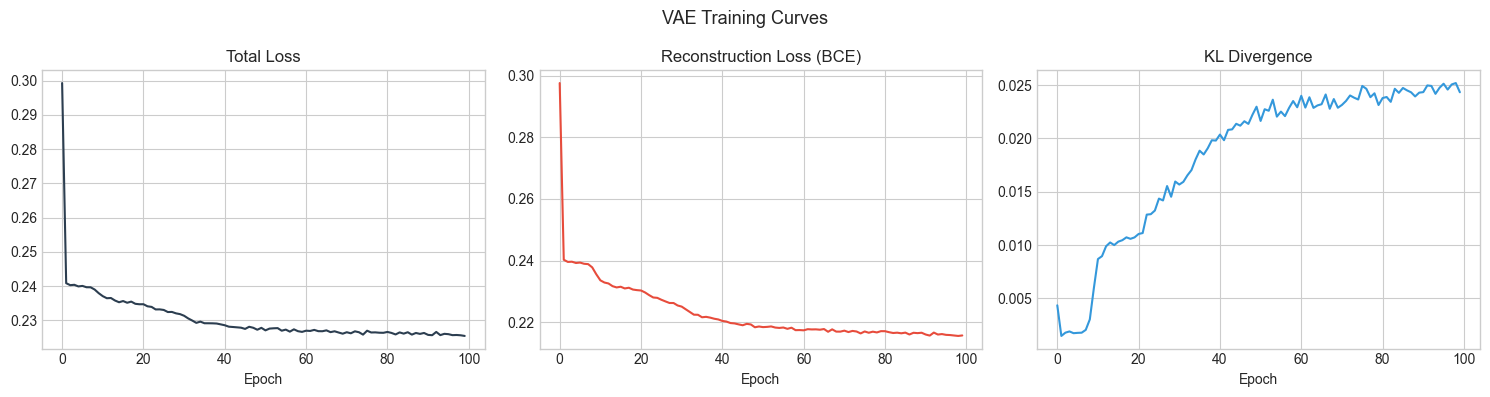
\includegraphics[width=0.5\textwidth]{Figuras/vae.png} 
  \caption{Dataset~1:VAE Training Curves}
\end{figure}

Another model which showed good performance and became a baseline for Dataset~2 and 3 is \textbf{Deep Convolutional Autoencoder} (ConvAE). The encoder applies three blocks of convolution, batch normalization, ReLU, and max-pooling, reducing a 3-channel input image down to a 128-dimensional latent vector. The decoder mirrors this with transposed convolutions to reconstruct the original image. Training uses MSE loss and Adam with early stopping. We use this model in all three datasets and treat it as the reference point against which more complex architectures are compared. 

To dive deeper into the autoencoder models and experiment, two more specialized variants were evaluated in the sensitivity study. \textbf{ResAttnAE} adds
residual skip connections and a channel-attention gate that re-weights feature maps before decoding, giving an attention-weighted reconstruction signal. \textbf{MemAE} introduces a fixed memory bank of prototypical patterns: the encoder output is soft-addressed into this bank, forcing the decoder to reconstruct only from stored prototypes and amplifying the error signal on any unseen distribution.

\subsubsection{Reconstruction Error as a Drift Signal}
Once a model is frozen, drift is measured as the increase in reconstruction error when
moving from reference images to target images. For a set of target images the
per-image error is
\begin{equation}
    e_i = \bigl\|\mathbf{x}_i - \hat{\mathbf{x}}_i\bigr\|^2,
    \label{eq:per_image_error}
\end{equation}
and drift is declared if the distribution of $\{e_i\}$ over the target period is
significantly higher than over the reference test set, assessed with a
Mann--Whitney~$U$ test at $\alpha=0.05$.

\begin{figure}[htbp]
  \centering
  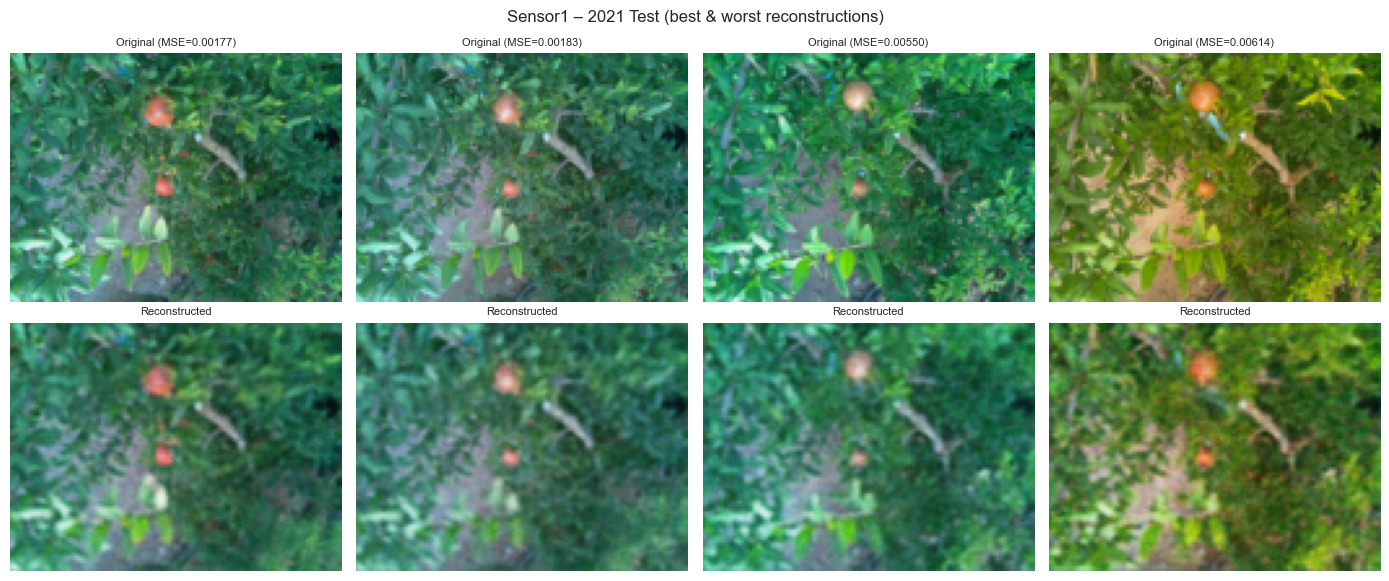
\includegraphics[width=0.5\textwidth]{Figuras/ex1.png} 
  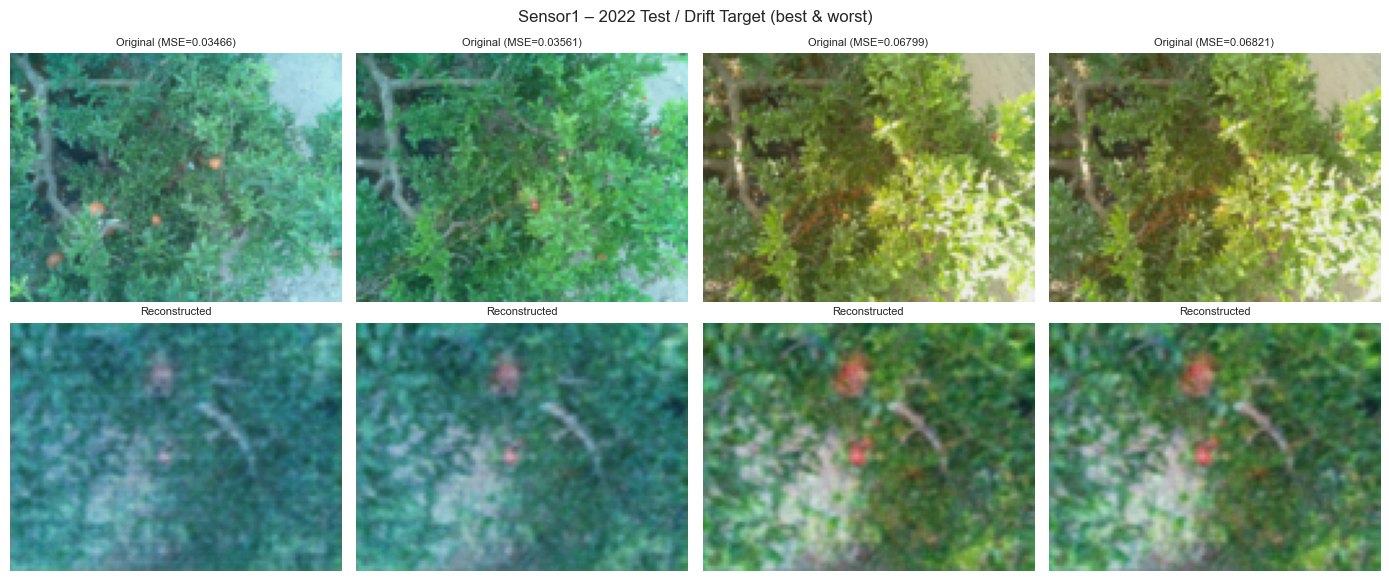
\includegraphics[width=0.5\textwidth]{Figuras/ex2.png} 
  \caption{Dataset~2:Sensor1 - 2021 Test(best and worst recontructions)}
\end{figure}

\subsubsection{Mean Time to Detection (MTTD)}
To make drift detection operationally meaningful, the MTTD is measured from the boundary between the reference and target period. A threshold $\tau$ is set at the $95$th percentile of reference reconstruction errors; images in the target stream are processed sequentially, and drift is declared the first time $k=3$ consecutive errors exceed $\tau$. Assuming a known capture rate $r$ (images per hour), MTTD in wall-clock time is:
\begin{equation}
    \text{MTTD} = \frac{n^*}{r},\qquad
    n^* = \min\bigl\{n : e_{n-2},e_{n-1},e_n > \tau\bigr\},
    \label{eq:mttd}
\end{equation}
and a cross-domain penalty factor $\phi = \bar{e}_\text{tgt}/\max(e_\text{ref})$
(capped at $2.0$) summarises how much harder the model struggles in the new domain.


\subsection{Sensitivity and Correlation Analysis}
To understand how robust the reconstruction signal is, a threshold sweep from the $50$th to the $98$th percentile quantifies precision, recall, F1, and MTTD at every operating point. Bootstrap confidence intervals ($B=1000$ resamples, $95\,\%$ CI) provide uncertainty estimates for each metric. Finally, to test whether the signal is genuinely structural rather than a proxy for surface illumination, six environmental
variance metrics (brightness, contrast, saturation, edge density, Shannon entropy, and colour divergence) are regressed against per-image reconstruction error using Pearson,
Spearman, and Kendall correlations alongside mutual information. A low correlation across all measures is taken as evidence that the autoencoder is responding to deeper distributional change rather than to easily-corrected photometric variation.

\begin{figure}[htbp]
  \centering
  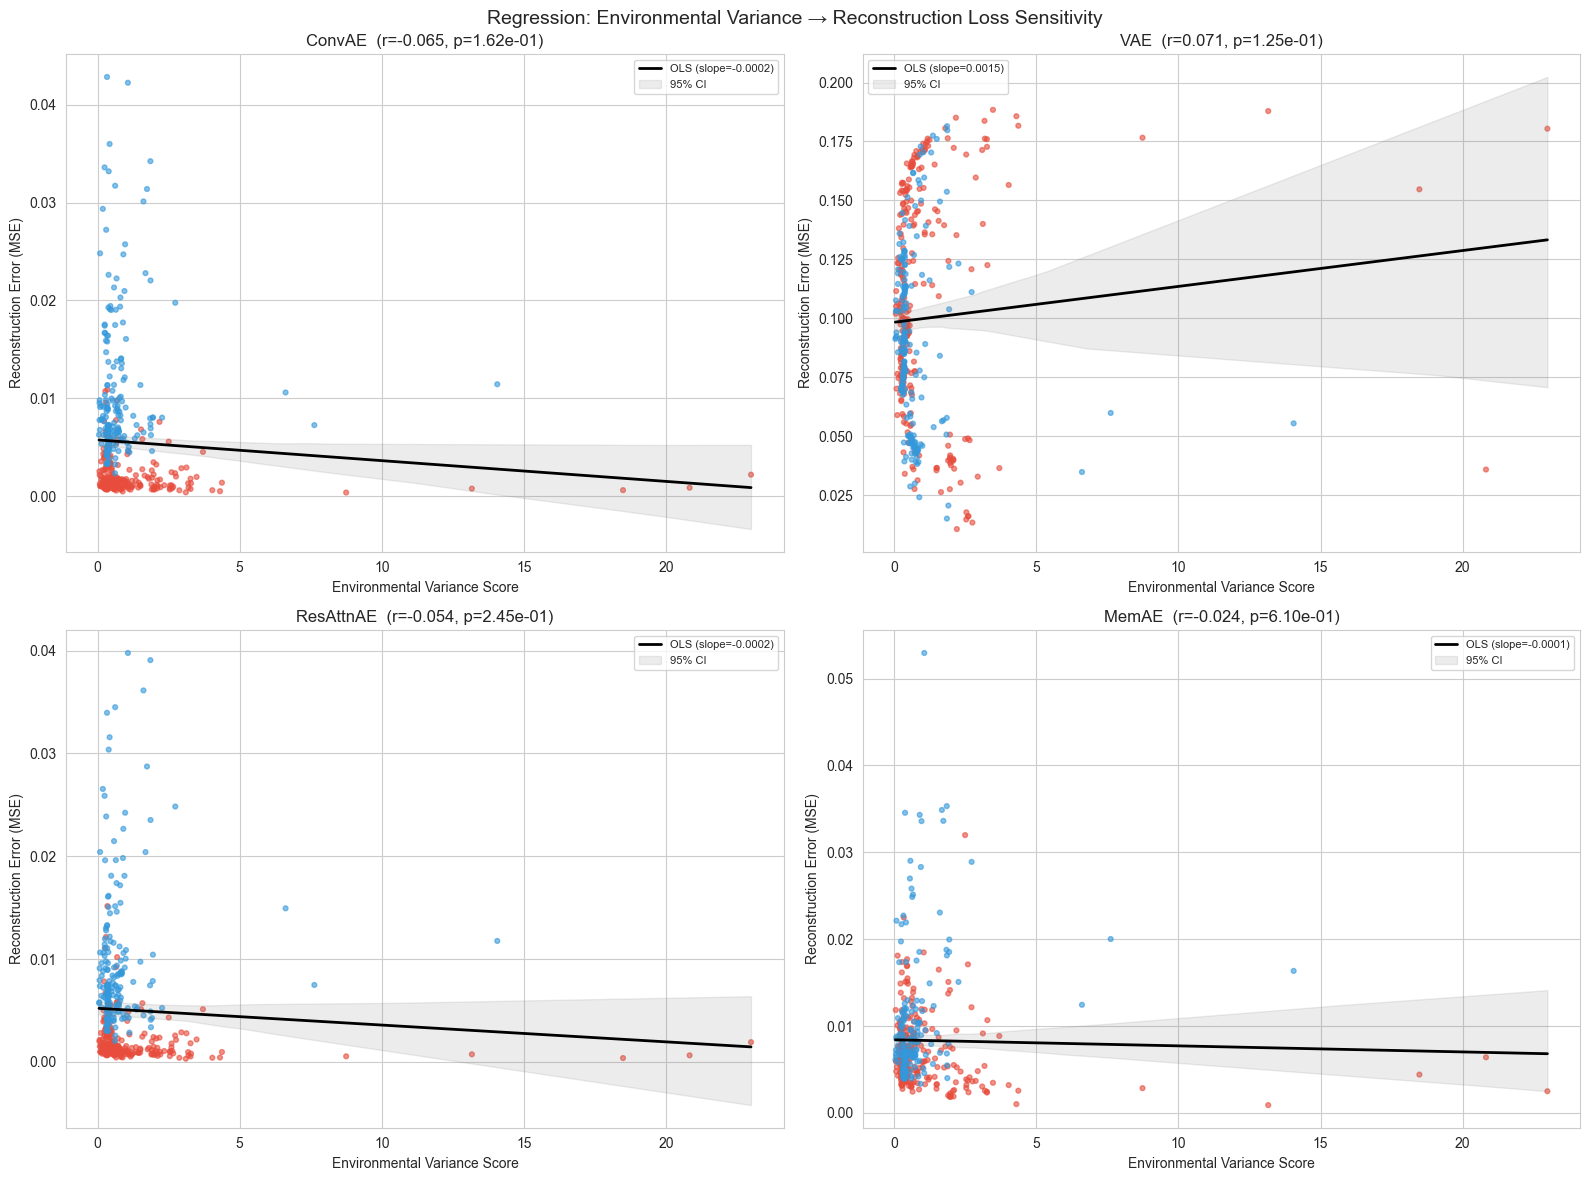
\includegraphics[width=0.5\textwidth]{Figuras/dataset3.png} 
  \caption{Dataset~3:Environmental Varience in Reconstruction Loss Sensitivity}
\end{figure}


\section{Results}

Taken together, the outcomes across all three datasets show that the proposed framework can detect meaningful distributional change in highly different IoT imaging environments. From subtle seasonal variation in urban street cameras to large biological changes in agricultural monitoring and rapid shifts in pest surveillance, the models consistently identified drift without relying on any labeled drift examples during training. Every result reported in this chapter therefore reflects the system’s ability to learn normal patterns and recognize when those patterns begin to change.

The latent space drift detection pipeline identified an overall drift score of \textbf{27.62\%}, which falls into the \emph{Moderate Drift} category, with a confidence score of \textbf{0.90}. Although the detected drift was relatively mild, it was statistically consistent across all 128 latent dimensions. Each dimension independently rejected the hypothesis that the Q1 and Q3 distributions were the same, confirming that a real distributional shift had occurred. Morever, the results of temporal drift tracking show that drift is worsening over time which is clear indication of sensor aging.

\begin{figure}[htbp]
  \centering
  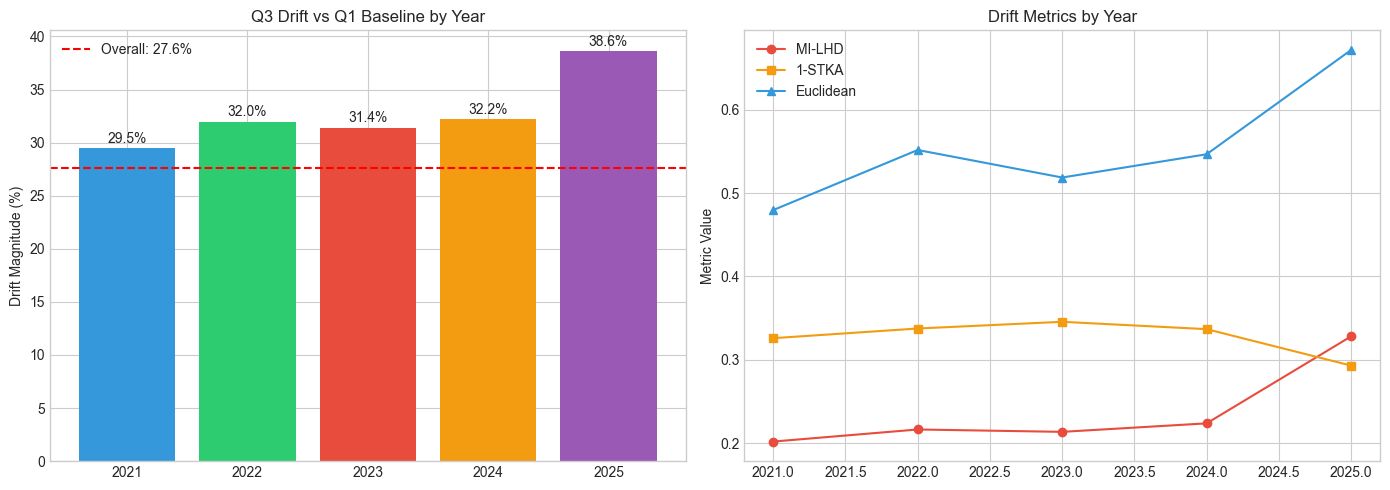
\includegraphics[width=0.5\textwidth]{Figuras/worsening.png} 
  \caption{Dataset 1 temporal drift tracking results}
\end{figure}


The second dataset produced the strongest and most consistent drift signal. All three models detected statistically significant drift across all 9 sensors, giving a \textbf{100\%} detection rate. When comparing the 2021 reference season with the 2022 target season we can see that the average reconstruction error increased substantially across all models:

\begin{figure}[htbp]
  \centering
  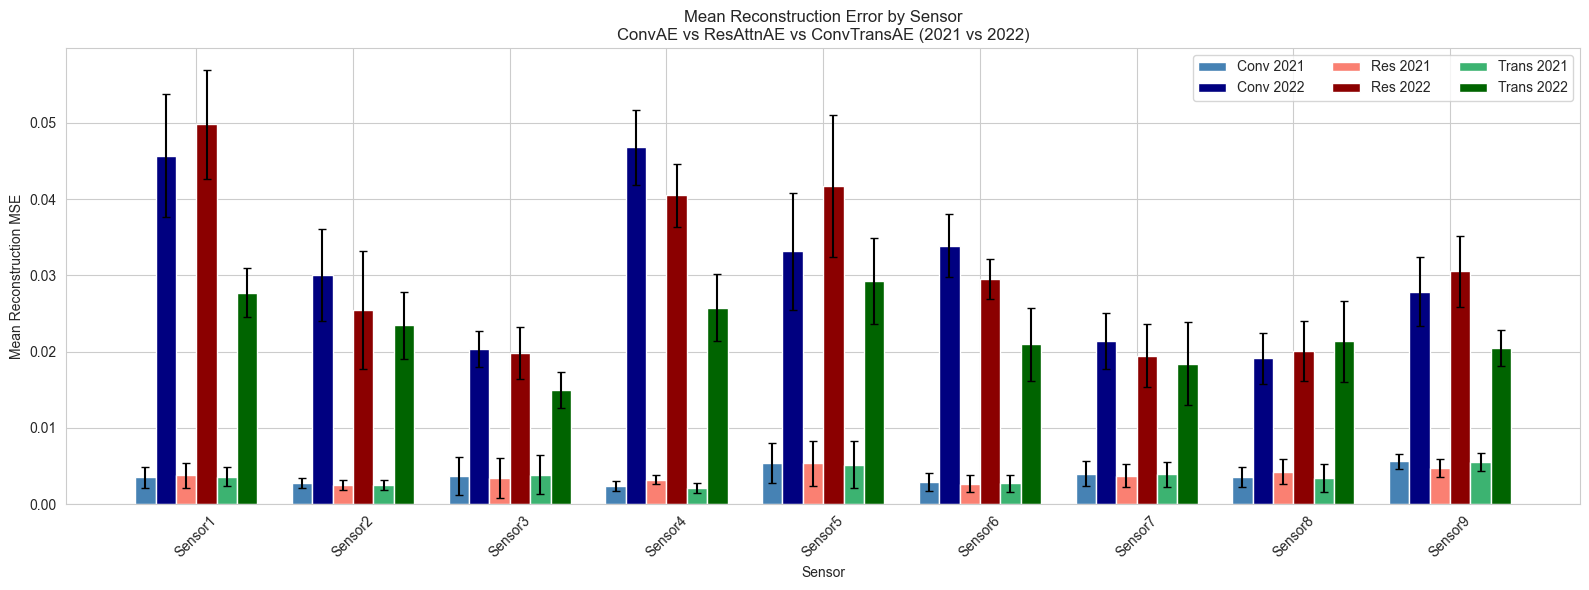
\includegraphics[width=0.5\textwidth]{Figuras/histograms.png} 
  \caption{Dataset~2:Mean reconstruction error by sensor}
\end{figure}

These increases indicate that the visual characteristics of the orchard changed dramatically from one year to the next. This is biologically plausible given the natural changes in tree growth, fruit development, pruning cycles, and seasonal conditions. Perhaps most importantly, all three architectures, despite learning in different ways, detected the same pattern of drift. That agreement greatly strengthens confidence that the detected changes reflect real environmental change rather than model specific behavior. Training stability was also strong, with final validation losses for all sensors remaining below \textbf{0.006}, indicating that the models learned stable representations of normal conditions before drift occurred.

In the Dataset~3 which is smallest by sample size, ConvAE detected a \textbf{+125.6\% increase} in reconstruction error when moving from Q3 (summer, reference) to Q4 (autumn, target), a highly significant result ($p = 1.35 \times 10^{-12}$). Using the 95th-percentile reference threshold, the system raised its first alert after just \textbf{14 frames - approximately 66 hours} - into the new season, demonstrating rapid real-world responsiveness. Furthermore, the four-model sensitivity analysis (Table~\ref{tab:ds3_models}) further highlighted the pipeline's strength:
\begin{table}[h]
\centering
\caption{ Dataset 3: Model Comparison (1,000 Bootstrap Iterations)}
\vspace{0.4cm}
\label{tab:ds3_models}


\begin{tabular}{
>{\raggedright\arraybackslash}p{1.5cm}
>{\centering\arraybackslash}p{1.5cm}
>{\centering\arraybackslash}p{0.5cm}
>{\centering\arraybackslash}p{0.5cm}
}
\toprule
\textbf{Model} & \textbf{ROC-AUC} & \textbf{Best F1} & \textbf{Drift (\%)} \\
\midrule

\textbf{ConvAE} & \textbf{0.891} & 0.554 & \textbf{+179} \\

\textbf{ResAttnAE} & 0.871 & \textbf{0.956} & +150 \\

\textbf{MemAE} & 0.557 & 0.241 & +22 \\

\textbf{VAE} & 0.323 & 0.053 & -22 \\

\bottomrule
\end{tabular}
\end{table}

\noindent
ConvAE and ResAttnAE both delivered excellent discrimination (ROC-AUC $> 0.87$), with ResAttnAE reaching a best-case F1 of \textbf{0.956} , which is obviously a near-perfect separation of normal and drifted images when the threshold is tuned. Crucially, reconstruction error was essentially \emph{uncorrelated} with environmental variance (Pearson $|r| \leq 0.07$ across all models), confirming that the drift signal reflects genuine distributional change in scene content rather than simple lighting variation.

\section{Analysis and Validation}

After analysing results its clear now that the project set out to detect and characterise unsupervised data drift in IoT imagery streams without relying on any labels performed quit good. Across all three datasets, the goal was clearly met. Every model on every dataset detected a statistically significant distributional shift between the reference and target periods, and the direction and magnitude of the shift matched the expected seasonal or inter-annual pattern. Importantly, the system identified drift without ever seeing labelled drift events during training and the only supervision was the temporal boundary between reference and target.

The results tell a coherent story across the three deployment contexts:

\begin{itemize}
  \item \textbf{Dataset~1} exhibits mild, expected drift that is partially seasonal
    and partially attributable to hardware ageing.  A drift score of \textbf{27.6\%} with a
    confidence of 0.90 is actionable but not alarming — it justifies periodic
    model recalibration rather than an emergency retraining.

  \item \textbf{Dataset~2} shows dramatic inter-annual drift, with reconstruction
    errors rising by \textbf{$60$–$80\%$} across all nine sensors.  This magnitude is
    biologically plausible: a pomegranate tree looks very different in July versus
    October, and 2022 had a different phenological progression than 2021.  The fact
    that all three architectures agreed on the direction of drift while differing in
    magnitude supports the view that the shift is real and robust, not a modelling
    artefact.

  \item \textbf{Dataset~3} presents the most nuanced picture.  The mean Q3-to-Q4
    drift of +126\% is genuine seasonal change, but the per-trap breakdown reveals
    that trap replacements (a known operational event) superimpose abrupt visual
    discontinuities on top of the gradual seasonal trend.  The \textbf{MTTD} of \textbf{14 frames (66 hours)}
     means the system would raise an alert within three days of the season
    change — fast enough to be practically useful.
\end{itemize}



\section{Discussion and Conclusion}

When started this project, the core problem felt almost invisible --- cameras keep running, models keep predicting, and nobody notices that the world the sensors see has quietly become a different place. That invisibility is exactly what makes feature drift dangerous in long-running IoT systems, and it is what motivated every design decision in this pipeline. So, what did we actually find?
 The short answer is: drift is real, it is detectable without a single label, and how fast we catch it depends heavily on where we deploy. The longer answer is what makes these results interesting.

Through many experiments the results across all three datasets revealed that hidden feature drift in IoT imagery can be detected in a meaningful, trustworthy way without any labels with the help \textbf{authoencoders}. The fact that multiple models consistently detect drift in the same direction, across different environments and architectures, suggests the signals are grounded in real environmental changes rather than modeling artifacts. The validator and per‑camera analysis further strengthen trust by separating likely environmental drift from sensor faults or configuration issues, using metadata such as GPS consistency, brightness trends, fault flags, and confidence scores. This makes the pipeline not only sensitive but also practical: operators can see where drift occurs and get a simple explanation of why, rather than reacting to generic alerts.

Overall, the research demonstrates that unsupervised autoencoders can form the core of an end‑to‑end drift monitoring system for long‑running IoT deployments. The pipeline is both interpretable—through reconstruction loss, MI‑LHD, STKA, and KS‑based metrics—and transferable across domains, which makes it suitable for real‑world monitoring when labeled data is scarce or unavailable.

\textbf{Future work} can focus on automating the validator logic further, for example by training a lightweight classifier on metadata and metrics to label drift events (e.g., “environmental,” “sensor fault,” or “artificial artifact”). Moreover, the suggested unsupervised method can be compared with other unsupervised classical benchmark methods in the IoT drift detection field to understand how effective it is compared with the newest existing methods\cite{nine}. 





\begin{thebibliography}{9}
\bibitem{one} 
Online Machine Learning from Non-stationary Data Streams in the Presence of Concept Drift and Class Imbalance: A Systematic Review. (2024). Journal of Information and Communication Technology, 23(1), 105-139.
\bibitem{two} 
S. G. Moumtzidis, G. Ditzler, and A. C. Souza, “Concept Drift Detection Methods Based on Different Weighting Strategies,” International Journal of Machine Learning and Cybernetics, 2024.

\bibitem{three}
M. Lu, A. Liu, and J. Gama, “Concept Drift in Streaming Data: A Systematic Literature Review,” Knowledge-Based Systems, vol. 195, 2020.

\bibitem{four}
G. Ditzler, M. Roveri, C. Alippi, and R. Polikar, “One or two things we know about concept drift—a survey on monitoring in evolving environments. Part B: locating and explaining concept drift,” 
Frontiers in Artificial Intelligence, vol. 7, 2024.

\bibitem{five}
A. Khamis, S. Aly, and M. Youssef, “Drift Detection Analytics for IoT Sensors,” IEEE Internet of Things Journal, vol. 8, no. 12, pp. 9812–9824, 2021.

\bibitem{six}
A. Elshawi, S. Sakr, and T. Hacid, “Enhancing IoT Sensors Precision Through Sensor Drift Calibration With Variational Autoencoder,” IEEE Sensors Journal, vol. 23, no. 4, pp. 4567–4578, 2023.

\bibitem{seven}
Renjie Chu, Peiyuan Jin, Hanli Qiao, Quanxi Feng. Intrusion detection in the IoT data streams using concept drift localization[J]. AIMS Mathematics, 2024.

\bibitem{eight}
J. Audibert, P. Michau, A. Li, and E. V. Ruiz, 
“An encode-then-decompose approach to unsupervised time series anomaly detection on contaminated training data,” 2025.

\bibitem{nine}
S.~Greco, B.~Vacchetti, D.~Apiletti, and T.~Cerquitelli, ``Unsupervised Concept Drift Detection from Deep Learning Representations in Real-time,'' \textit{IEEE Transactions on Knowledge and Data Engineering (TKDE)}, 2025.

\bibitem{ten}
Hinder, F., Vaquet, V., and Hammer, B. (2024a). One or two things we know about concept drift-a survey on monitoring in evolving environments. Part A: detecting concept drift. Front. Artif. Intell. 7:1330257. doi: 10.3389/frai.2024.1330257

\bibitem{eleven}
A Multi-Year Urban Streetlight Imagery Dataset for Visual Monitoring and Spatio-Temporal Drift Detection. https://arxiv.org/html/2512.12205v1#S5

\bibitem{twelve}
S. Kang, Y. Park, J. Lee, and B. Mozafari,
“ODIN: Automated drift detection and recovery in video analytics,”
Proc. VLDB Endow., vol. 15, no. 11, pp. 2683–2696, 2022.

\bibitem{thirteen}
S. Kornblith, M. Norouzi, H. Lee, and G. Hinton,
“Similarity of neural network representations revisited,”
in Proc. Int. Conf. on Machine Learning (ICML),
2019, pp. 3519–3529.

\bibitem{fourteen}
J. Giménez-Gallego, J. Martínez-del-Rincon, P. J. Blaya-Ros, H. Navarro-Hellín, P. J. Navarroand R. Torres, ‘Dataset of pomegranate tree (Punica granatum L. 'Wonderful') image times series’. Zenodo, Mar. 18, 2024. doi: 10.5281/zenodo.10829695.

\bibitem{fifteen}
A. Kargar, D. Zorbas, M. Gaffney, B. O'Flynnand S. Tedesco, ‘Image Dataset of Brown Marmorated Stink Bug (BMSB) or Halyomorpha Halys (HH)’. Zenodo, 2025. doi: 10.5281/zenodo.16088064.



\end{thebibliography}

\end{document}